\input{../../template.ltx}

\usepackage{graphicx}

\begin{document}

\osuetitle{3}

\section*{Aufgabenstellung}

\textbf{Shared-Integrator}

Schreiben Sie zwei Prozesse zum verteilten Integrieren des bestimmten Integrals
$$\int^{\mathtt{max}}_{\mathtt{min}} \frac{x^2}{4}$$

\begin{verbatim}
    SYNOPSIS
        server min max n_per_packet numpackets
        integrate
\end{verbatim}

Es gibt einen Server-Prozess und beliebig viele Integrier-Prozesse. Der Server
teilt den zu integrierenden Bereich in \emph{numpacket} Pakete auf. Die
Integrier-Prozesse übernehmen jeweils einzelne Pakete, integrieren diese, und
geben das Teilergebnis an den Server zurück. Jeder Integrier-Prozess teilt sein
Paket wiederum in \emph{n\_per\_packet} Teile auf und verwendet zum Integrieren
ein einfaches Riemannsummen-Integral:
$$\int^b_a f(x) = \frac{b-a}n \cdot \sum_{i=1}^{n} f\left(a + i\cdot \frac{b-a}{n}\right)$$

Ist ein Integrier-Prozess mit einem Paket fertig, holt er sich vom Server ein
neues. Es kann also durchaus weniger als \emph{numpackets} Integrier-Prozesse
geben. Wenn das letzte Teilergebnis eingesammelt wurde, gibt der Server das
Ergebnis auf \emph{stdout} aus.

\subsection*{Beispiel}

$n\_per\_packet = 10, numpackets = 3$

Das Integral wird in diesem Fall in drei Pakete zerlegt, die vom Server-Prozess
an die Integrier-Prozesse ausgeteilt werden. Jeder Integrier-Prozess zerlegt
dann das erhaltene Paket in zehn Teile, von denen dann die Riemannsumme
berechnet wird.

\begin{center}
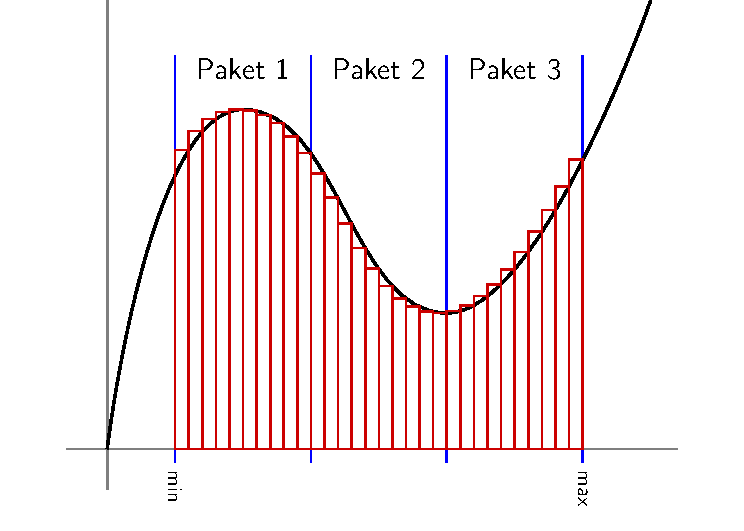
\includegraphics[height=6cm]{integfigure.pdf}
\end{center}

\subsection*{Hinweis}
Die Kommunikation zwischen dem Server-Prozess und den Integrier-Prozessen soll
über einen Shared-Memory-Bereich stattfinden. Die Anzahl der Clients ist nicht
beschränkt; sie können zu beliebigen Zeitpunkten gestartet werden und
terminieren jeweils wenn kein neues Paket verfügbar ist. Das Integrieren soll
beginnen, sobald der erste Integrier-Prozess verfügbar ist. Überlegen Sie sich
ein geeignetes Synchronisations-Schema für diese Aufgabe.

\subsection*{Anleitung}
Schreiben Sie zwei Programme, die die Prozesse mittels einer
Client/Server-Struktur realisieren. Achten Sie auf saubere Terminierung.

\osueguidelinesthree

\end{document}
